\section{Defining and Applying the AES Technique}
\label{SEC:approach}

\begin{figure}[t]
  \center{}
  \fbox{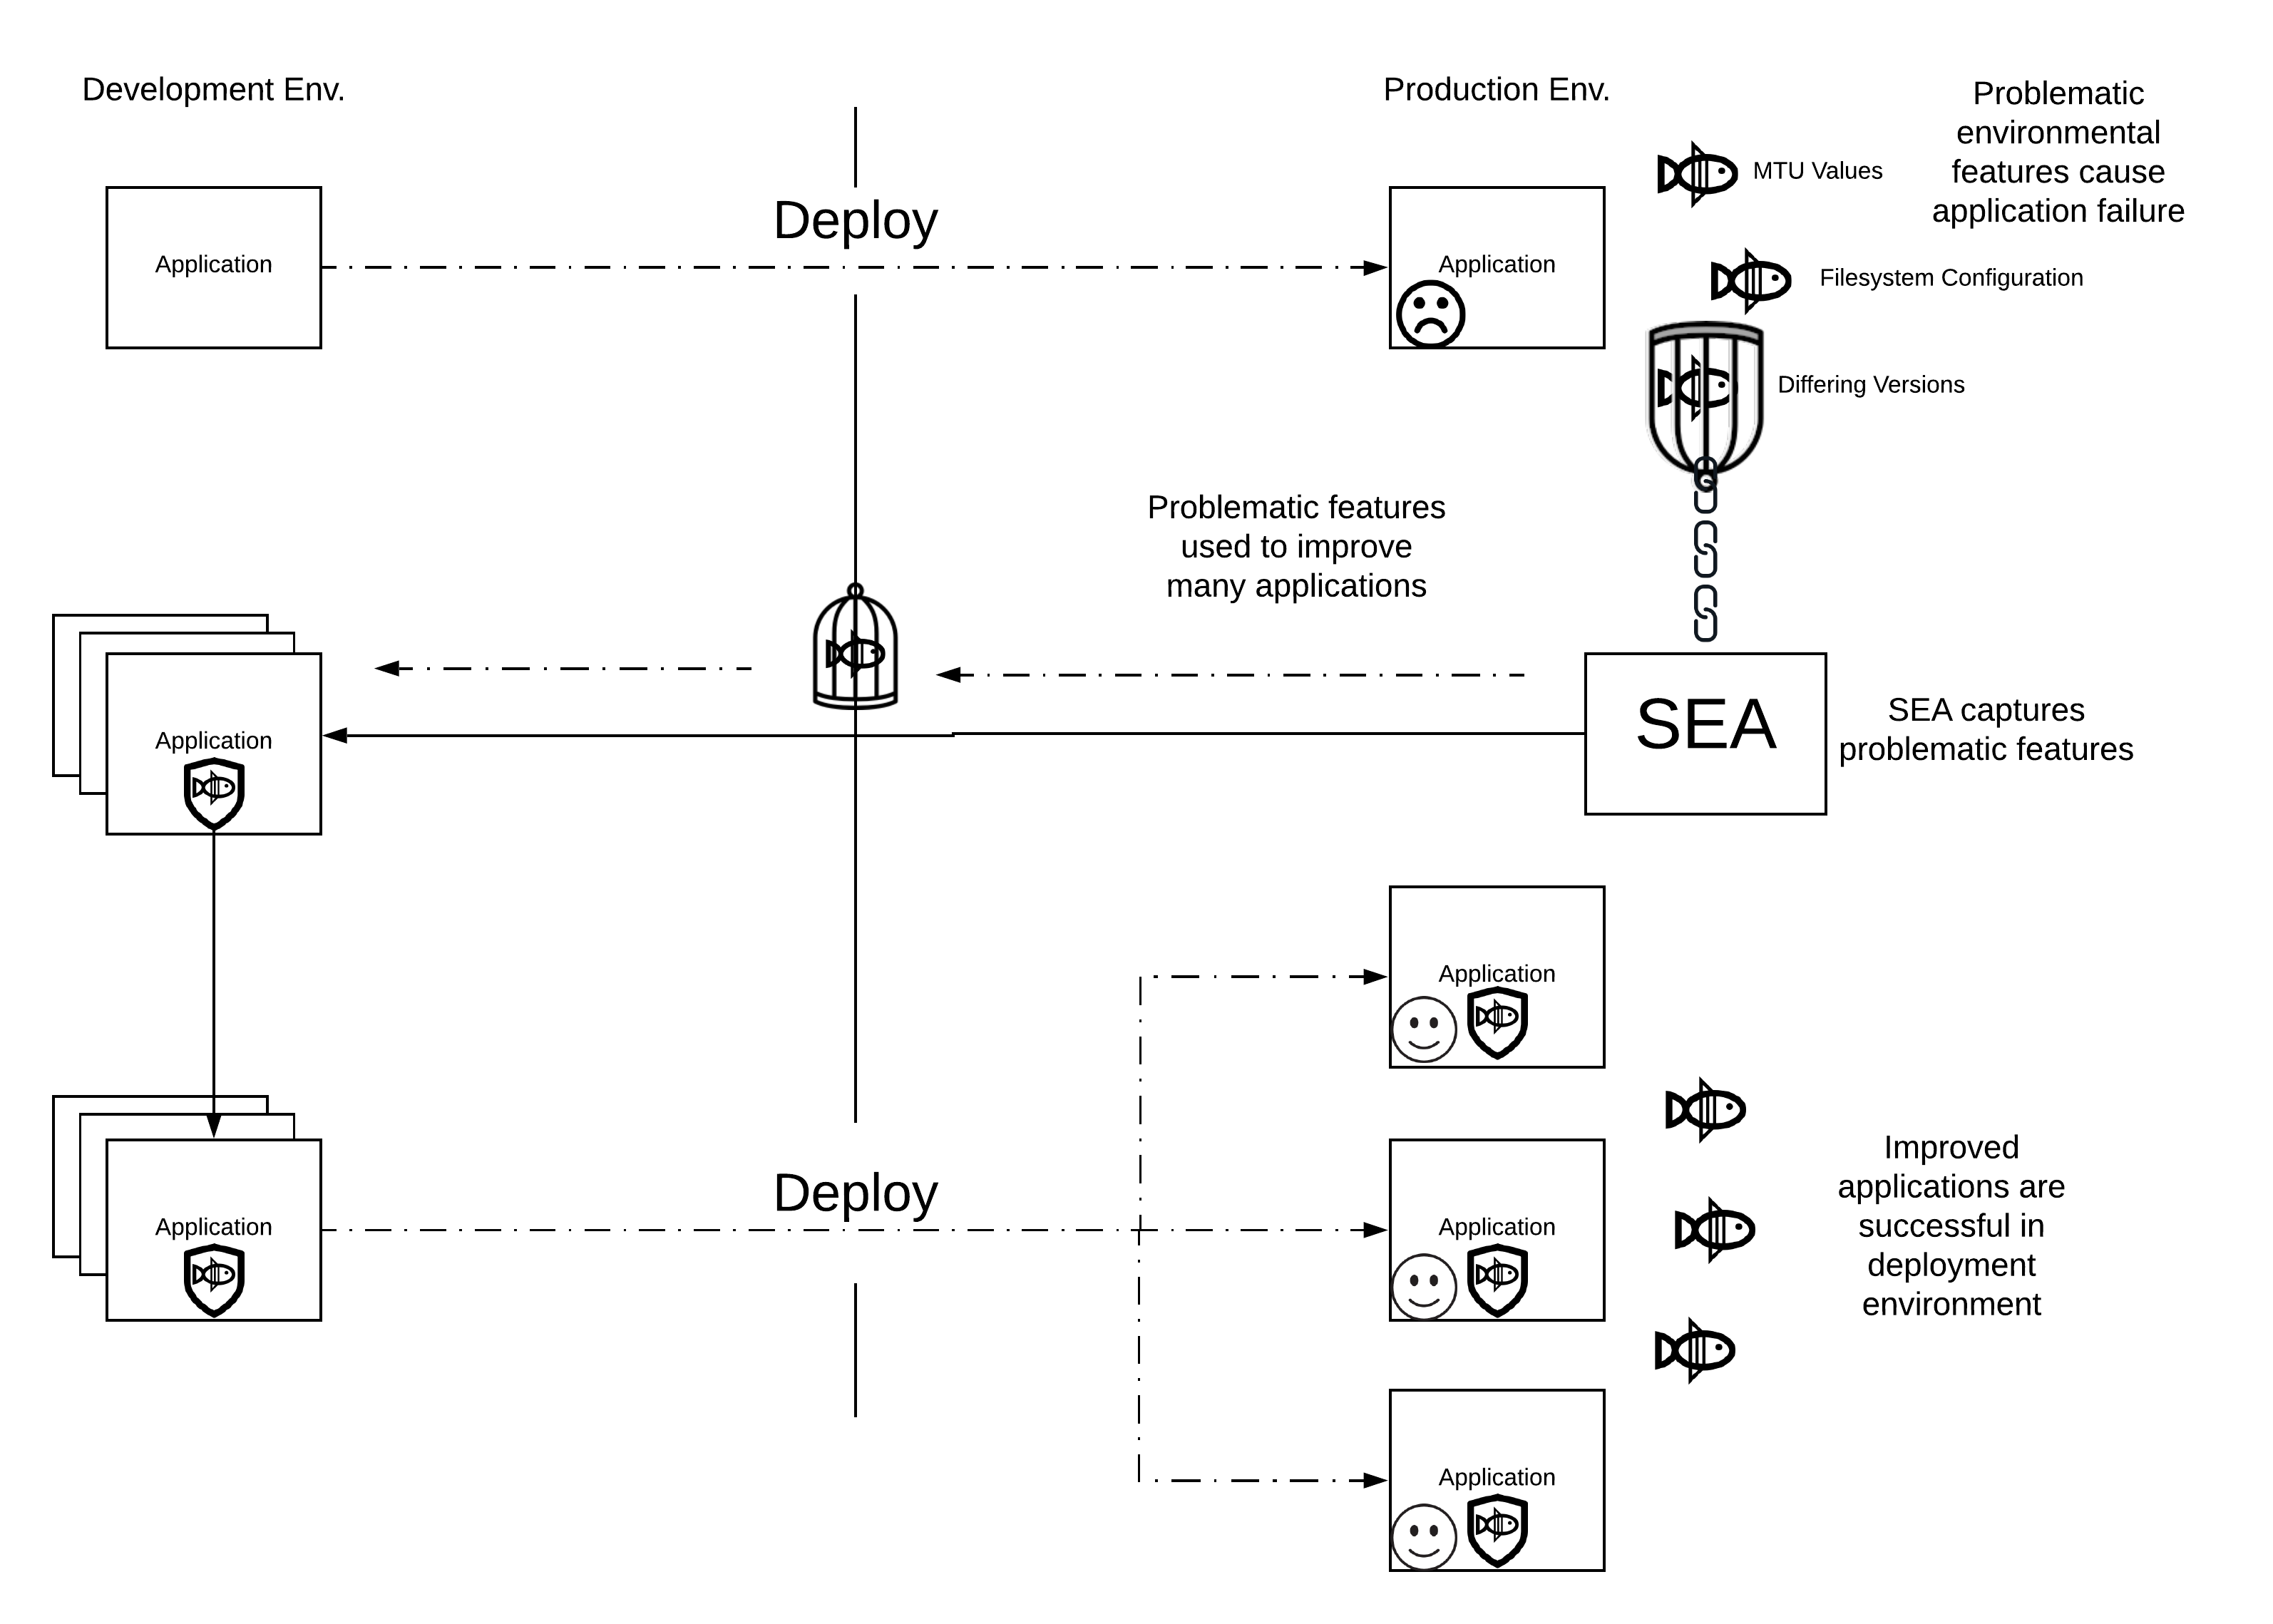
\includegraphics[scale=.37]{images/approach}}
  \caption{Diagram illustrating CrashSimulator's approach}
  \label{figure:approach}
\end{figure}

\begin{figure*}[t]
  \center{}
  \fbox{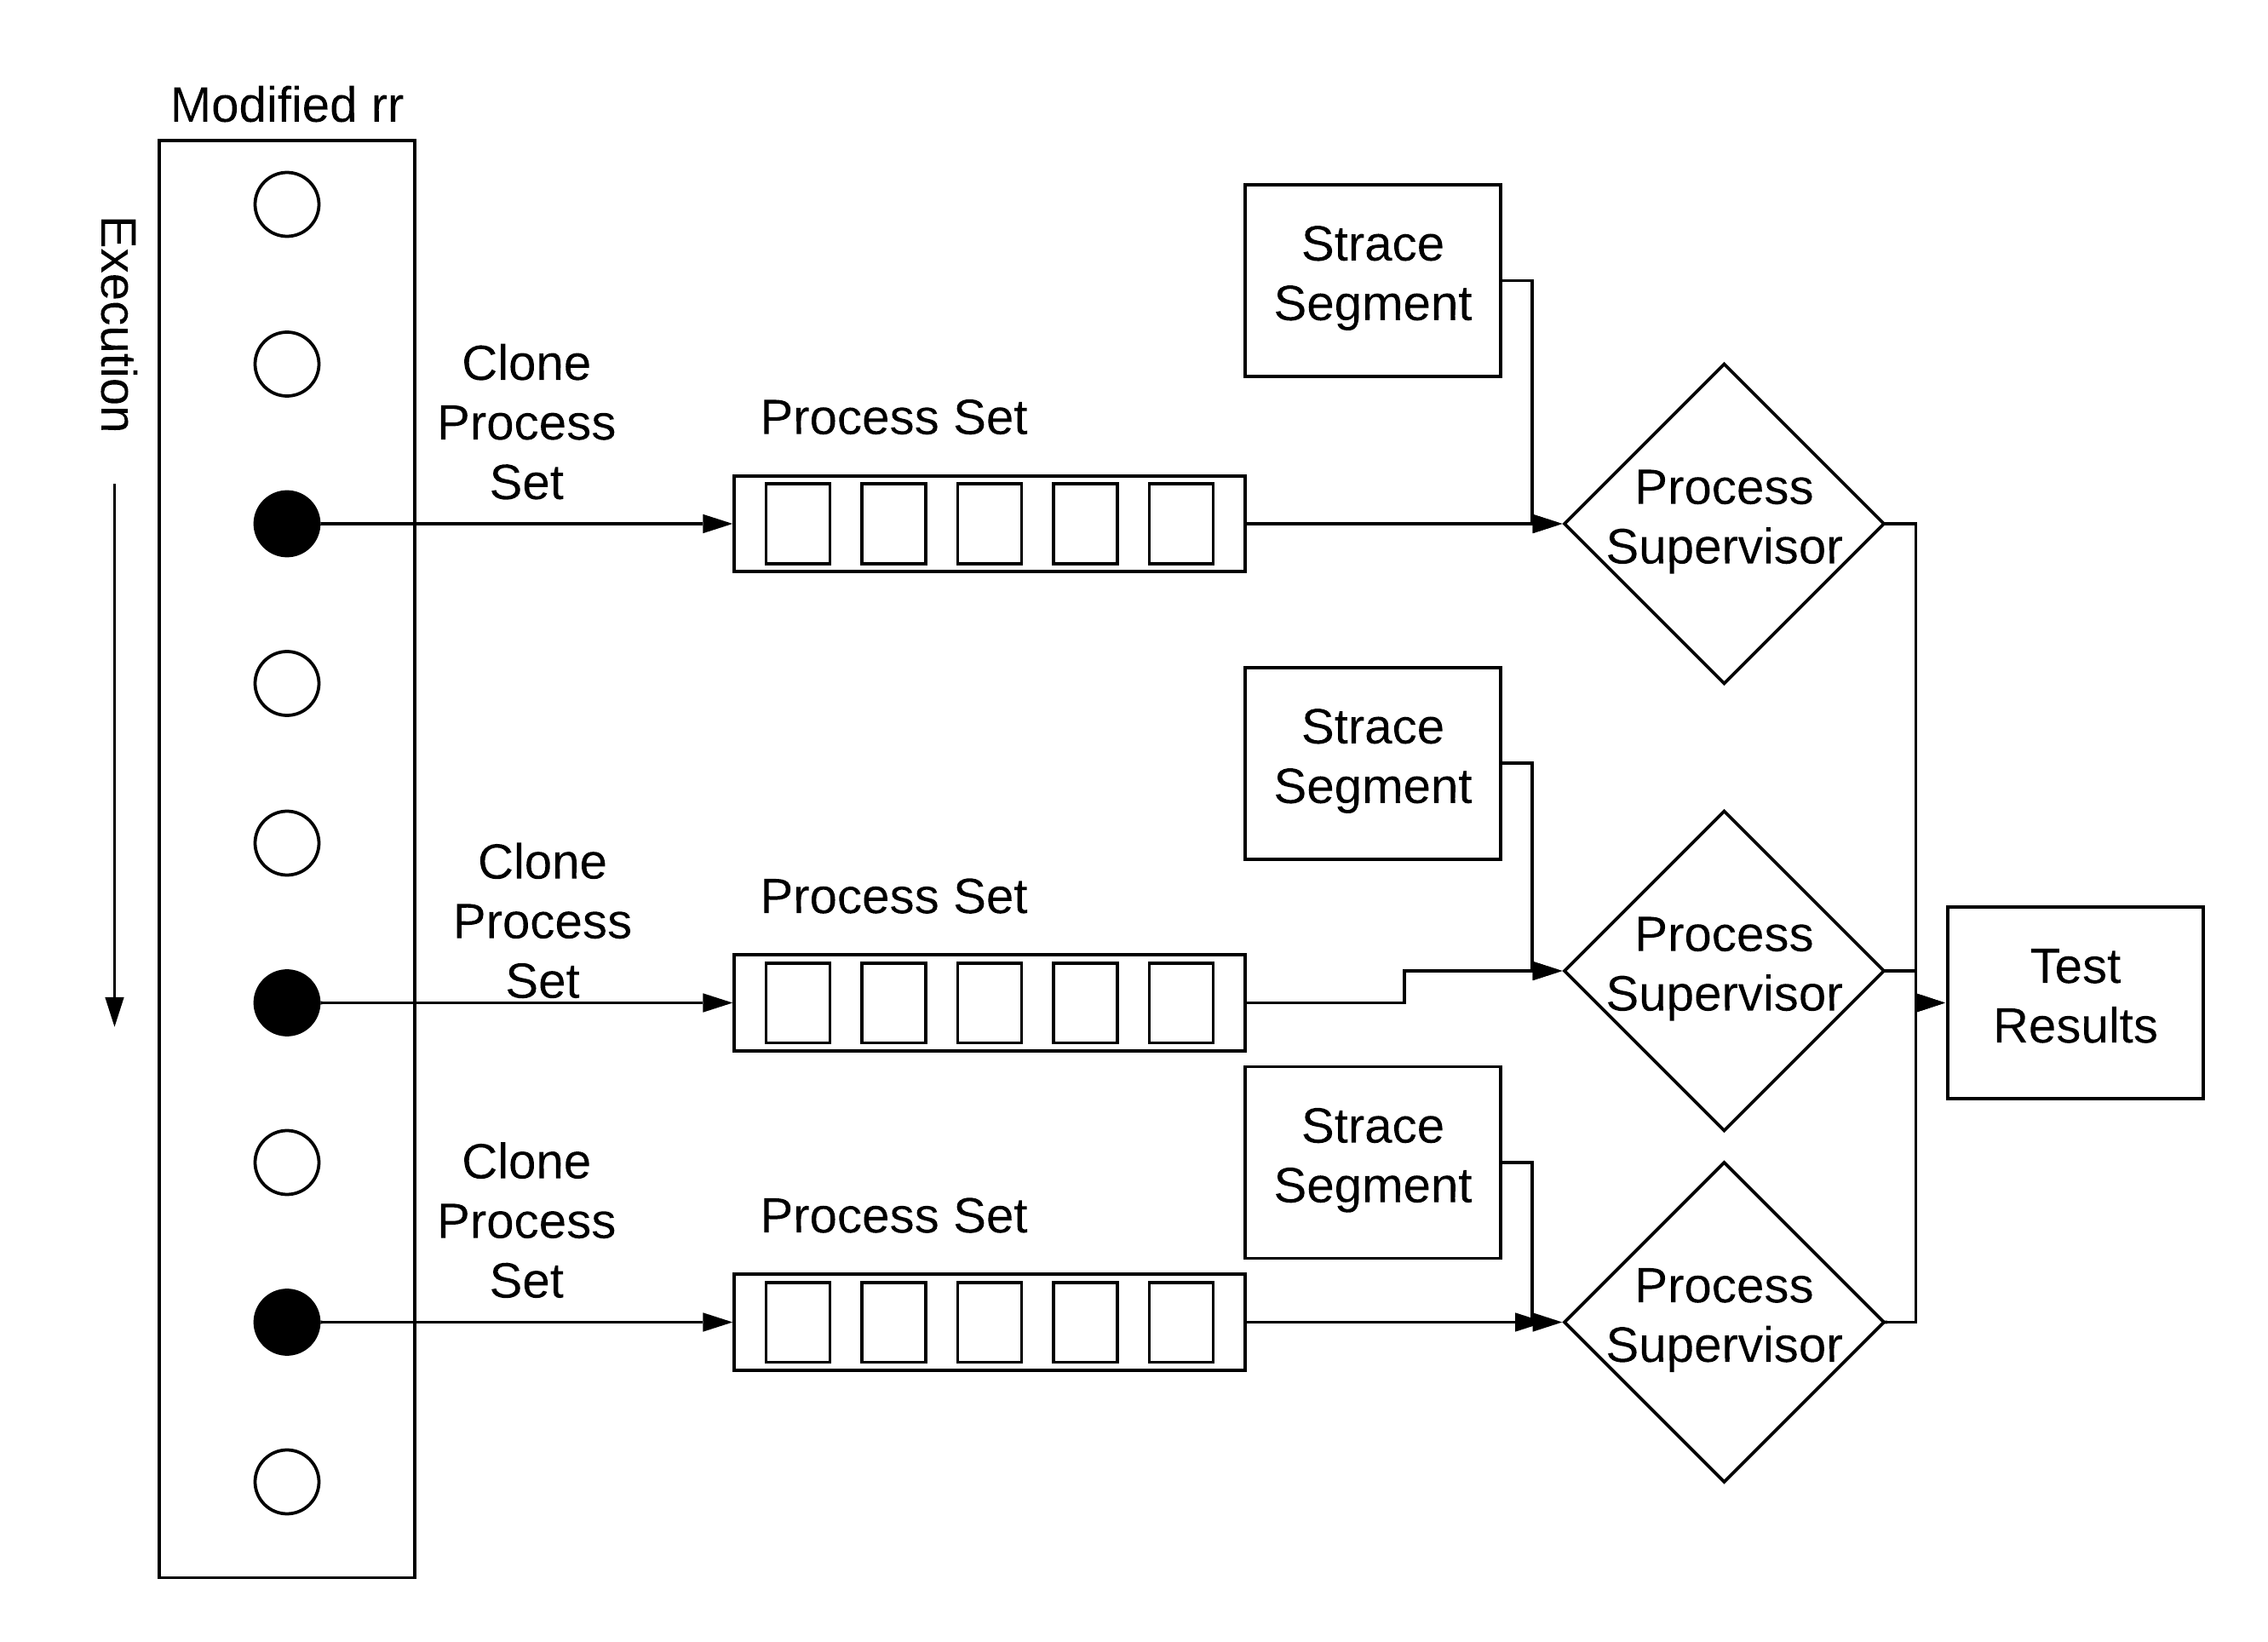
\includegraphics[scale=.65]{images/architecture}}
  \caption{Diagram illustrating CrashSimulator's Architecture.  During the
    course of a single rr execution, clone process sets are generated at
    specific rr events.  A CrashSimlator supervisor process attaches to
    these process sets and uses a strace-style system call listing to feed
    subsequent system call activity and inject unusual environmental
    conditions.}
  \label{figure:architecture}
\end{figure*}

As mentioned earlier,
the anomalous environment simulation(AES) technique
offers a reliable way to identify bugs
that could arise from interaction with a given environment.
In this section,
we will break down the steps of the technique,
and then introduce a tool called CrashSimulator,
which we built as a concrete implementation of AES.
We also describe a second technology
called Process Set Cloning
that evolved during our work on CrashSimulator.
Process Set Cloning describes an enhancement made to
the {\tt rr} debugger on which CrashSimulator was built
that allowed us to generate copies of the set of processes underlying an
application at opportune moments during replay.


\subsection{Stepping through AES}

The first step in implementing AES
is selecting an anomaly or anomalies
against which you wish to test an application.
Anomalies can be collected
by examining the failures of other applications
in a target deployment environment,
through public bug trackers,
or by using other tools that can identify
potentially problematic behavior in other domains~\cite{Zhuang_NSDI_2014,
rasley2015detecting}.
Selecting bugs public trackers
is ideal if you wish to determine
whether or not an application
is vulnerable to a widely publicized bug.
The chosen anomalies are then examined
to determine how they change an application's communications
with its environment
compared to a normal execution and why.
Once teased out,
these differences delineate
a set of modifications
that must be made to an application's communications
in order to simulate the chosen anomaly or anomalies.
As an example,
consider an anomalous environment
where access to a required file is denied because of
the environment's file security configuration.
This anomaly results in attempts to access the file,
such as calls to {\tt fread()},
or the {\tt read()} system call,
which fail with an error stating that access to the file is denied.
The ``modification'' required to simulate this anomaly
is to change the results of similar accesses
in a test execution
to return ``access denied.''

The second step in AES
is identifying
a way to monitor an application's communication
with its environment.
This can be implemented
by such means as
redirecting function calls,
observing memory access,
monitoring network activity,
or intercepting system calls.
Looking at the parameters,
return values,
and orderings
of an application's communications
can indicate
when would be an appropriate time to simulate an anomaly.
Monitoring communications
in this fashion
has the added benefit
of allowing us to find obvious situations
where an application will fail
to handle certain environmental features,
since such failures will be visible.
Consider an application that fails to check whether or not
a file already exists
before destructively writing to it.
The absence of this check
would be problematic in environments where the file already exists,
as it will be blindly overwritten.
The sequence of communications
the application makes when writing to the file
will make it obvious that this check has been neglected.
As such,
no simulation is required to identify the presence of a bug.

In cases such as the one described above,
the AES technique could stop at this point.
However, in most scenarios,
the last two steps ---
simulation and response analysis ---
will be required.
In the third step,
the implementer
interposes on communications
and makes the modifications necessary
to simulate the presence
of an environmental anomaly.
This could be accomplished by
influencing the results of function calls or system calls,
strategically altering memory values,
or some other method
of presenting modified communications to an application.
In the simplest case,
simulating an anomaly only requires
the modification of a single value.
In more complex cases,
large numbers of diverse communications
need to be interdicted and altered
in order to correctly simulate an anomaly.
For example,
simulating an erratic system clock
requires that all efforts
to access the clock
be modified to reflect the chosen aberration.

Lastly, the fourth AES step
is to analyze an application's response
to a simulated anomaly.
This is accomplished
by evaluating an its communications
after exposure is completed.
The simplest conclusion to draw
is whether or not the application
has made an effort to respond
to the anomaly,
a determination that can be made based
on the assumption
that such a response will yield
different program paths (and therefore different communications).
If the application
does not alter its behavior, it has not
correctly handled this flaw.
Alternatively,
if the application does deviate,
it is likely
an action has occurred to handle the simulated condition.
This simple yes or no approach
is often sufficient
to classify application behavior.

One limitation of the above strategy
is that it can result in false negatives
should an application change its behavior
but still not handle the anomaly correctly.
These false negatives can be addressed
by more detailed analysis
of the application's post simulation behavior.
Before testing,
a user must know
what a correct response
to an anomaly looks like.
This ``known good'' behavior can be found
by looking at standards and documentation
that describe best practices for handling an anomaly
in a given environment,
or by examining how applications that correctly
deal with the anomaly do so.
Consider the case where a {\tt close()} system call fails.
Retrying the call may not be the correct action,
depending upon the environment in question.
AES can be used to determine if an application
has handled the failure correctly
by examining post-simulation communications in detail,
and taking into account the correctness of retrying the call.

\subsection{CrashSimulator: A Concrete AES Implementation}

Evaluating AES in a real-world fashion requires a concrete implementation
of its four components.  Evaluating AES in a real-world fashion requires a
concrete implementation of its four components. We built this
implementation into a tool we call CrashSimulator. To be able to evaluate
how effectively CrashSimulator performs—and to test, a series of tests were
conducted using a prototype build on rr version 5.2.0 running on a
32-bit Linux kernel running distributed with Ubuntu 16.04 LTS. Our
modifications to rr were carried out in C++ and the CrashSimulator
supervisor was implemented in ZZZZ lines of Python 2.7 code with a YYYY
line C extension that allows it to interact with processes using the Ptrace
API. This version of CrashSimulator is available as a Docker container and,
due to some operating system configuration being necessary, is most easily
installed in this fashion.

Below, we explain the process of creating CrashSimulator, highlighting a
few central principles that guided our design decisions. The first such
decision was to operate at the system call level, rather than manipulating
calls to library functions, memory accesses, or other points where we could
influence an application's communications. Making this choice provided us a
few key advantages. First, there is already robust tooling in the Linux
kernel that allows for the interception and modification of system call
results and side effects. Additionally, Linux system call semantics are
well defined which simplifies implementation. Finally, operating at this
level allows CrashSimulator to test applications written in any language
that can execute Linux system calls.

Work then turned to gathering a corpus of anomalies to test applications
against.  These anomalies (which are further discussed
in Section~\ref{SEC:evaluation})
were collected by examining public bug trackers,
the source code of major portable applications, and the capabilities of
tools like NetCheck~\cite{Zhuang_NSDI_2014}
and CheckAPI~\cite{rasley2015detecting}.  These anomalies were converted
into sets of modified responses
that simulate the presence of an anomaly when
appropriately presented as the results of system calls.
This process required manual effort and expertise.  However,
much like
the effort involved in constructing a unit test to check for correct
behavior in a piece of code, we found that this initial outlay of
user skill and effort was paid back, as
we were able to use its products
repeatedly over time to test many different applications.

We carried out the second step of AES, communication monitoring, by
recording application executions
using a modified version of the {\tt rr}!!CITE!!
debugger.  This modification allowed
a {\tt strace}-style
system call recording to be output alongside {\tt rr's} normal recording
format, providing
a complete log of an applications system call activity.
With this information, we could
easily identify opportunities to simulate anomalies.  As was
discussed earlier, simply observing these system calls was enough to
identify bugs-of-omission in many applications
(see Section~\ref{SEC:evaluation} for a more detailed explanation).

In implementing the anomaly simulation of AES
we actually developed
a second new technique
called {\it process set cloning}.
With the modification made to rr described above,
we now can generate copies of the set of
processes underlying an application at opportune moments during replay.
The {\tt rr} debugger manages
and can copy
the full set of these
so that users can test debugging
hypotheses without damaging the original.
Our modified version
extends this capability, by liberating process sets from {\tt
rr} so that they can be exposed to simulated anomalies.
This means that we can rely on {\tt rr}
to store the information necessary to perform enough of the
replay that must take place before the application reaches the
testing point.

Process sets generated in this fashion are created in a stopped state and
remain that way until they are attached to and utilized by a CrashSimulator
supervisor.  Each process set has its own supervisor process to test
its configured environmental anomaly.  The
supervisor wakes up its designated process set
and simulates any
subsequent system calls.
During the course of this simulation, the modified responses created in
step one are supplied where appropriate,
thus exposing the processes to the
anomaly being tested.
Supervisors can complete this
process independently of one another, which lends a
high degree of speed and
parallelism to the whole CrashSimulator testing process.

The primary means by which
CrashSimulator diagnoses bugs is
by observing whether or not an application
performs a different set of system calls than what is expected based on the
recording being replayed.  A ``divergence'' from the recording indicates
the application has changed its behavior and might be handling
the anomaly in question.  Following the recording precisely, in spite of
the simulated anomaly signals the possibility of a bug.

In cases where more detailed analysis of an application's response
is required, CrashSimulator can use a
technique called ``execution preservation'' to allow a process set to run
``off the end'' of the recording supporting it.  This technique uses
heuristics to generate false data to populate the results and
side effects of system calls the application makes in this state.  This
effort is necessary because resources like files on disk, file descriptors,
and sockets do not exist due to the nature of replay execution.  While
execution is being preserved, finite automata known as ``checkers`` examine
the system calls being made in order to make more detailed claims about the
application's response.  These checkers are discussed in more detail in our
evaluation.
